\section{The Approach}

\subsection{One Important Limitation}

\begin{frame}
  \frametitle{One Important Limitation}
  \centering
  \Large \textit{Unlike Pregel, graph topology is immutable.}
\end{frame}


\subsection{The Basic Idea: Combine GAS with Node Partitioning}

\begin{frame}
  \frametitle{The GAS Decomposition}
  The authors observed this pattern across many vertex programs.
  \begin{itemize}
    \item \textbf{Gather} an accumulated results from neighborhood.
    \item \textbf{Apply} the gathered result on the center node.
    \item \textbf{Scatter} accumulated information across the neighborhood.
  \end{itemize}
\end{frame}

\begin{frame}
  \frametitle{Node Partitioning}
  \begin{figure}
    \centering
    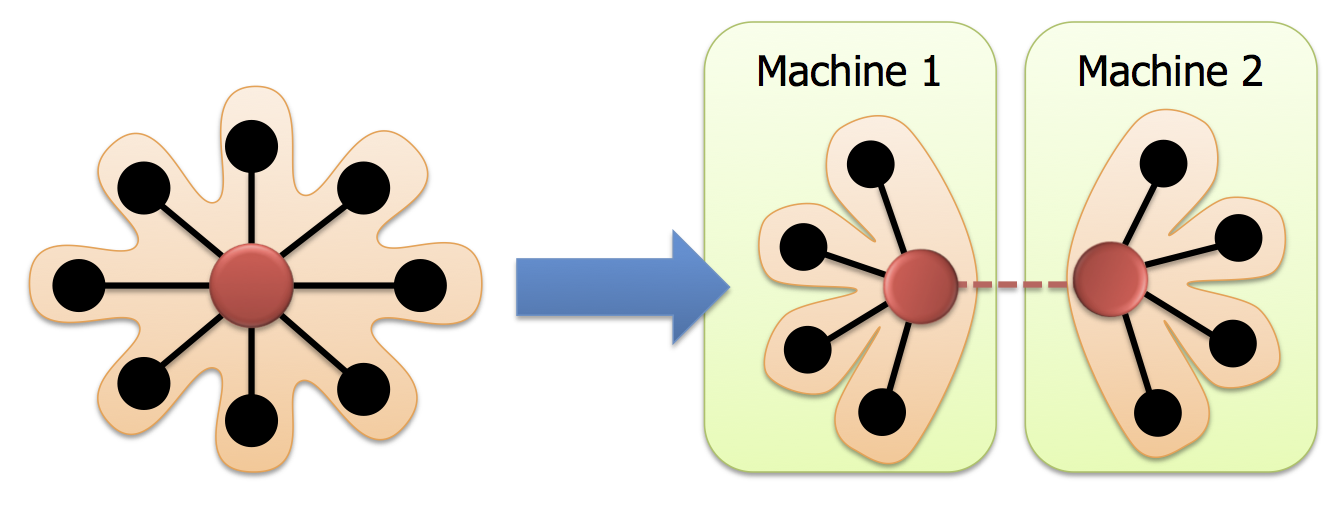
\includegraphics[scale=0.37]{gonzalez_osdi_2012_slide_13_simple}
    \caption{\cite[OSDI '12 Slides]{gonzalez2012powergraph-slides}}
  \end{figure}
\end{frame}

\begin{frame}
  \frametitle{The Key to PowerGraph's Optimizations}
  \centering
  Parallelize vertex programs as before, but also parallelize their
  sub-operations, scatter and gather. \textit{(Smaller critical sections!)}

  \begin{figure}
    \centering
    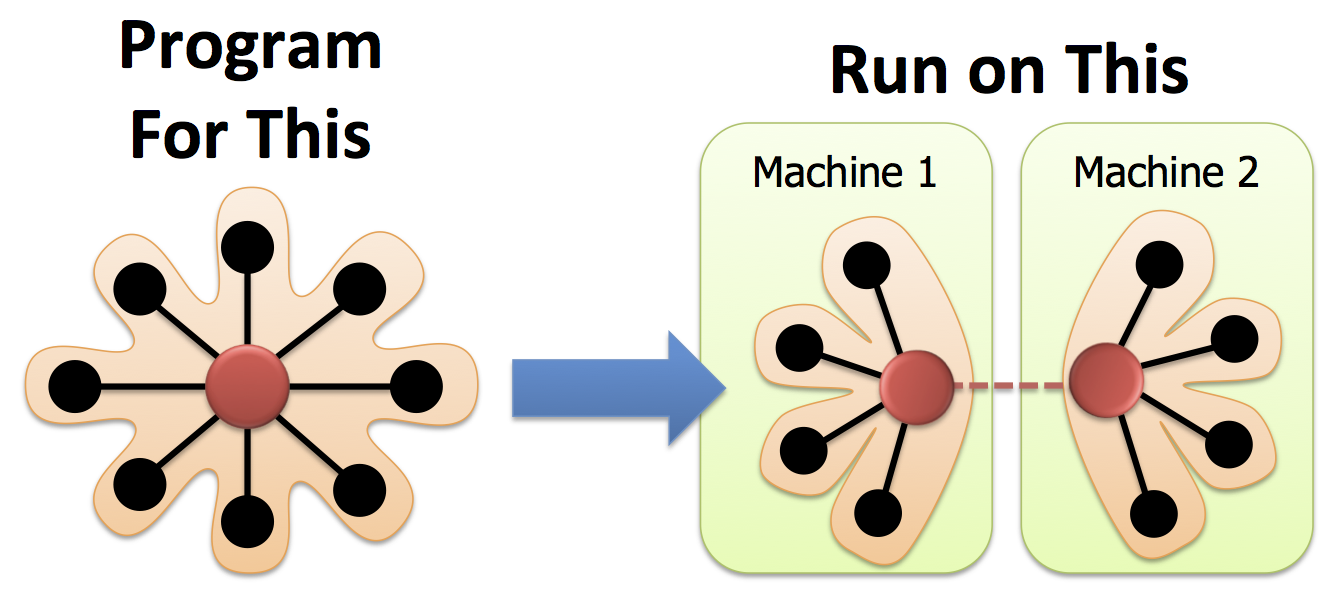
\includegraphics[scale=0.37]{gonzalez_osdi_2012_slide_13}
    \caption{\cite[OSDI '12 Slides]{gonzalez2012powergraph-slides}}
  \end{figure}
\end{frame}

\begin{frame}
  \frametitle{A Taste of the Results}
  \begin{figure}
    \centering
    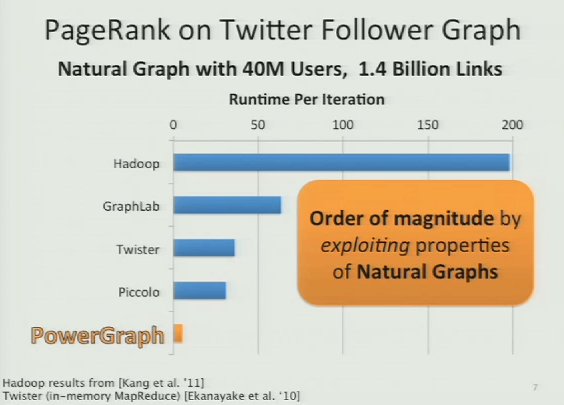
\includegraphics[scale=0.40]{gonzalez_osdi_2012_slide_7}
    \caption{\cite[OSDI '12 Slides]{gonzalez2012powergraph-slides}}
  \end{figure}
\end{frame}


\subsection{The PowerGraph Abstraction}

\begin{frame}
  \frametitle{The GAS Decomposition}
  \begin{figure}
    \centering
    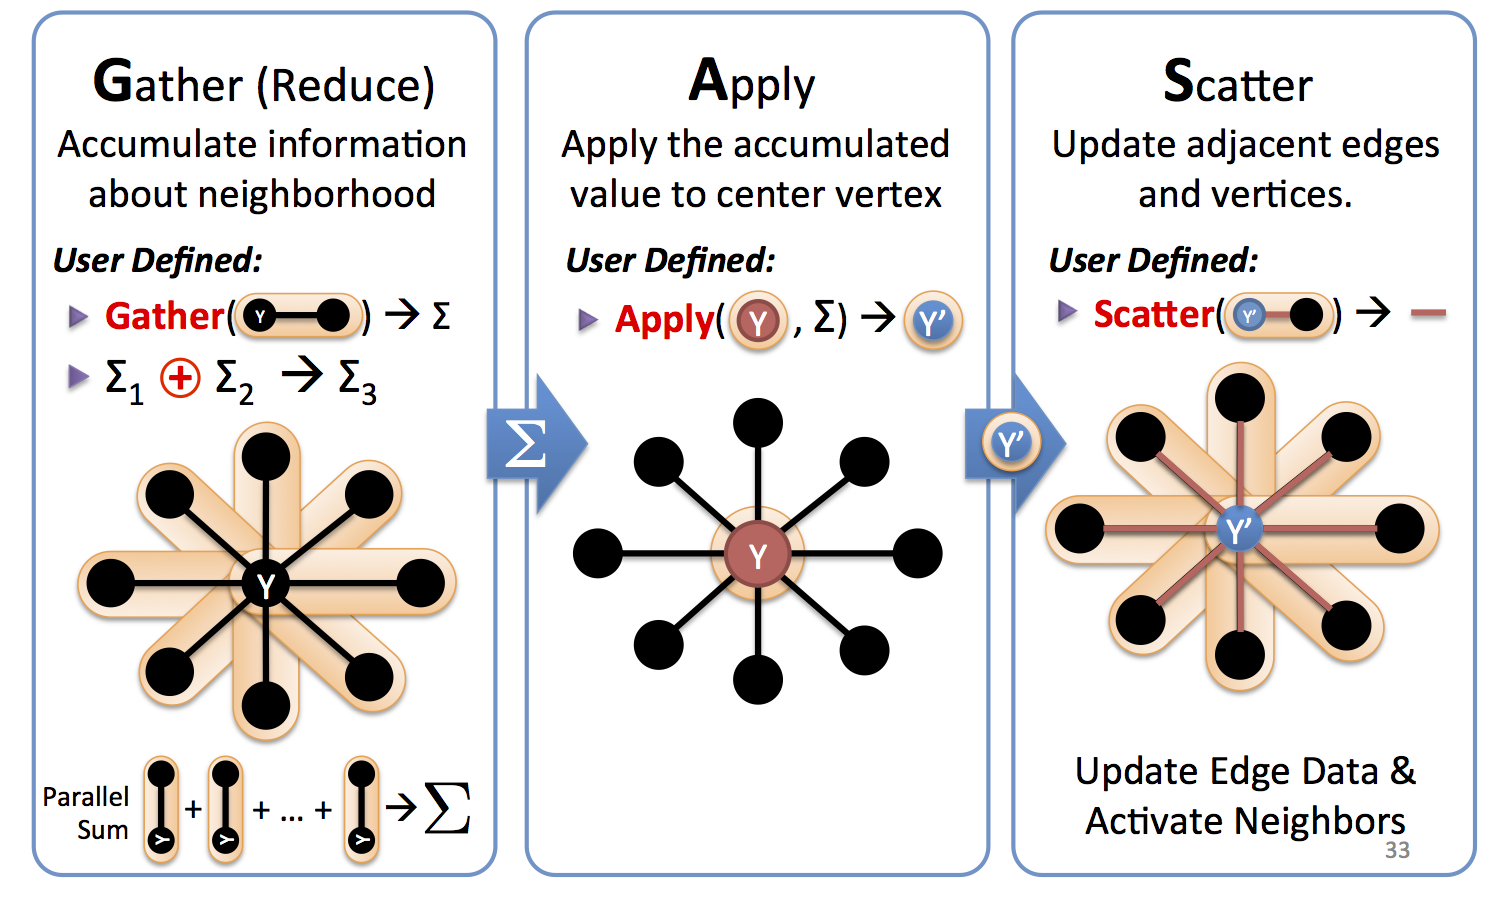
\includegraphics[scale=0.34]{gonzalez_osdi_2012_slide_33}
    \caption{\cite[OSDI '12 Slides]{gonzalez2012powergraph-slides}}
  \end{figure}
\end{frame}

\begin{frame}
  \frametitle{The PowerGraph Abstraction}
  PowerGraph lifts the GAS decomposition into the framework. The user implements
  each of these to make a vertex program.
  \begin{figure}
    \centering
    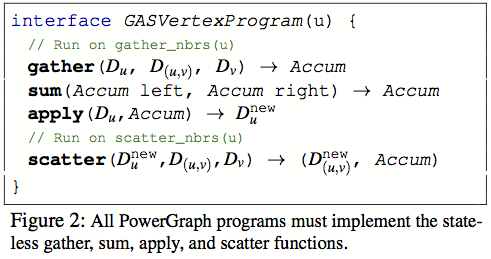
\includegraphics[scale=0.75]{gonzalez_osdi_2012_figure_2}
    \caption{\cite[OSDI '12]{gonzalez2012powergraph}}
  \end{figure}
\end{frame}

\begin{frame}
  \frametitle{Delta Caching}
  \begin{itemize}
    \item Might better be called ``cached gather accumulator with corrections.''
    \item A programmer-directed optimization, useful in some programs.
    \item \textbf{Idea:} When scattering to neighbor, optionally add a
          correction onto cached gather accumulator.
  \end{itemize}
\end{frame}

\begin{frame}
  \frametitle{Node Activation}
  \begin{itemize}
    \item Except for initial activation (of all vertices), activation is always
          explict in user's vertex program.
    \item A vertex can only be activated by itself or by one of its neighbors.
    \item \textbf{Rule:} A vertex program can activate vertices in
          \textbf{gather()}, \textbf{apply()}, or \textbf{scatter()}, but only
          on \textit{visible} vertices (i.e.\ vertices that are part of args).
  \end{itemize}
\end{frame}

\begin{frame}
  \frametitle{Sequential Semantics}
  The meaning of a vertex program given the user-defined ops:
  \begin{figure}
    \centering
    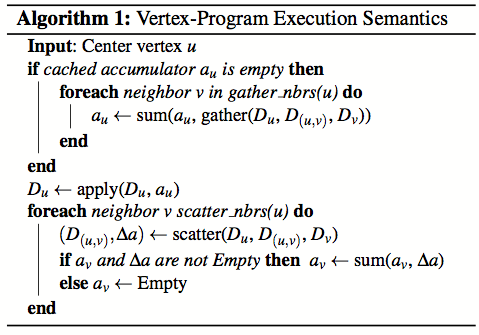
\includegraphics[scale=0.78]{gonzalez_osdi_2012_algorithm_1}
    \caption{\cite[OSDI '12]{gonzalez2012powergraph}}
  \end{figure}
\end{frame}

\begin{frame}
  \frametitle{\textit{Example:} Greedy Graph Coloring}
  \begin{figure}
    \centering
    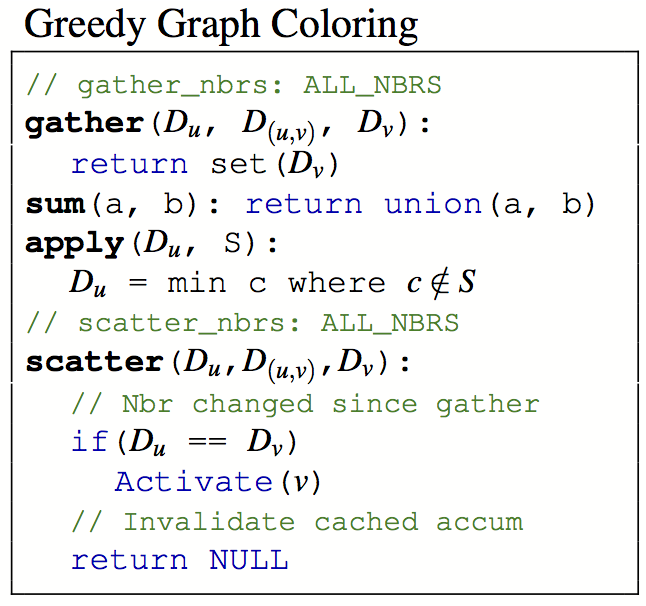
\includegraphics[width=0.45\textwidth]{gonzalez_osdi_2012_figure_3b}%
    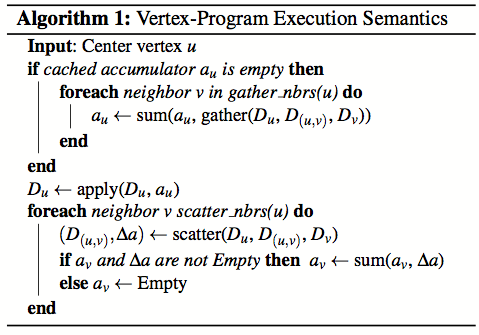
\includegraphics[width=0.55\textwidth]{gonzalez_osdi_2012_algorithm_1}
    \caption{\cite[OSDI '12]{gonzalez2012powergraph}}
  \end{figure}
\end{frame}


\subsection{Distributing the Graph and Computation}

\begin{frame}
  \frametitle{Edge-Cut vs Node-Cut Graph Partitioning}
  \begin{figure}
    \centering
    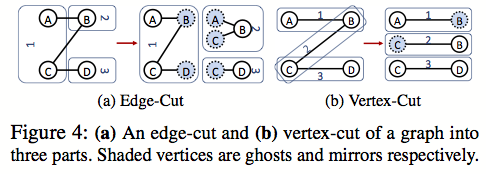
\includegraphics[scale=1.0]{gonzalez_osdi_2012_figure_4}
    \caption{\cite[OSDI '12]{gonzalez2012powergraph}}
  \end{figure}
\end{frame}

\begin{frame}
  \frametitle{A Vertex Program on a Cut Vertex}
  \begin{figure}
    \centering
    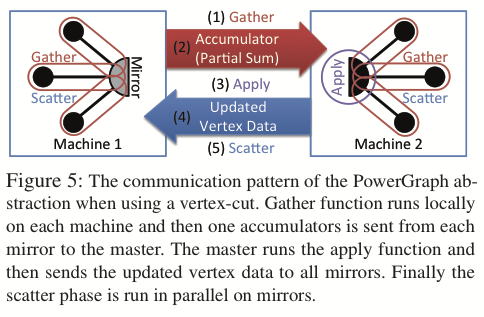
\includegraphics[scale=0.95]{gonzalez_osdi_2012_figure_5}
    \caption{\cite[OSDI '12]{gonzalez2012powergraph}}
  \end{figure}
\end{frame}

\begin{frame}
  \frametitle{Graph Partitioning Formalization and Algorithms}
  \begin{itemize}
    \item The authors formally describe an optimization problem for graph
          partitioning (balanced $p$-way vertex-cut), and two algorithms for
          finding approximate solutions (random and greedy).
    \item The authors argue that the vertex-cut model is ``highly effective''
          for both power-law graphs and regular graphs.~\cite[OSDI '12]{gonzalez2012powergraph}
    \item These are not covered in this presentation.
  \end{itemize}
\end{frame}


\subsection{An Example Vertex Program}

\begin{frame}
  \frametitle{\textit{Example:} Greedy Graph Coloring}
  \begin{figure}
    \centering
    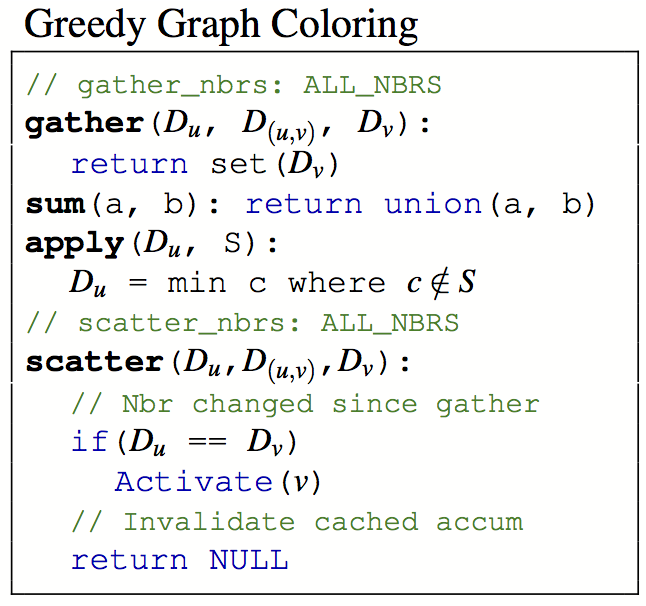
\includegraphics[scale=1.0]{gonzalez_osdi_2012_figure_3b}
    \caption{\cite[OSDI '12]{gonzalez2012powergraph}}
  \end{figure}
\end{frame}


\subsection{PowerGraph Runtime}

\begin{frame}
  \frametitle{Three Variants of PowerGraph's Runtime}
  \begin{itemize}
    \item \textbf{Bulk Synchronous:} Vertex program progress synchronized at
          both \textit{minor-steps} and \textit{super-steps}.
    \item \textbf{Asynchronous:} Mutations to graph are immediately visible by
          subsequent adjacent vertex programs.
    \item \textbf{Asynchronous Serializable:} \ldots
  \end{itemize}
\end{frame}

\begin{frame}
  \frametitle{Asynchronous Serializable}
  \textbf{Def:} A guarantee of \textit{serializability} is a guarantee that
    every possible parallel/distributed execution of vertex programs has a
    corresponding sequential execution.\footnote{\cite[OSDI '12]{gonzalez2012powergraph}}
\end{frame}

\begin{frame}
  \frametitle{Asynchronous Serializable}
  \centering
  Async+S is equivalent to GraphLab's \textit{edge consistency}.
  \begin{figure}
    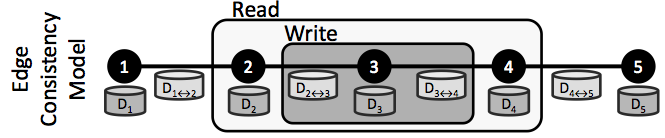
\includegraphics[scale=1.8]{low_vldb_2012_figure_2b}
    \caption{\cite[VLDB '12]{low2012distributed}}
  \end{figure}
\end{frame}


\subsection{}

\begin{frame}
  \centering
  \textbf{\Large Questions?}
\end{frame}
